\documentclass{ximera}

\addPrintStyle{..}

\begin{document}
	\author{Bart Lambregs}
	\xmtitle{Resonantie}{}
    \xmsource\xmuitleg



	%%%\section{Resonantie}

	% microgolfoven
	
	Het verschijnsel resonantie is je zeker bekend. Naar alle waarschijnlijkheid heb je ooit je kleine zusje geduwd op de schommel. Uiteraard deed je dat niet zomaar willekeurig maar met de juiste regelmaat. Je duwde wanneer ze net voorbij het hoogste punt bij jou was -- niet wanneer ze naar je toe kwam! Op die manier ging zij hoger en hoger en nam het plezier alleen maar toe. En dat totdat ze schrik kreeg omdat jij te ver ging \ldots
	
	We beschouwen een model waarin we een massa-veersysteem niet langer vrij laten trillen maar onderwerpen aan een periodieke aandrijvende kracht waarvan we de frequentie controleren. We hebben dan een gedwongen trilling. In ons model kunnen we natuurlijk allerlei soorten manieren van externe krachten steken maar om een differentiaalvergelijking te bekomen die toch ergens hanteerbaar is, nemen we een oscillerende kracht $F=F_0\cos\omega t$ waarin $F_0$ de maximale kracht is waarmee we trekken of duwen en $\omega$ de pulsatie waarmee we de kracht sinusoöidaal laten variëren. Ook voegen we ditmaal wrijving toe. We nemen een model waarin de wrijvingskracht recht evenredig is met snelheid $F_w=-cv$. Hierin is $c$ een coöefficiënt die de sterkte van de demping bepaalt. Het minteken zorgt ervoor dat de component van de wrijvingskracht steeds tegengesteld is aan de snelheid; de wrijvingskracht werkt de beweging altijd tegen. Zolang de snelheid niet te groot wordt, is dit een realistisch model. We vertrekken weer met de tweede wet van Newton:
	\begin{gather}
	F=ma\nonumber\\
	\Downarrow\nonumber\\
	-kx-cv+F_0\cos\omega t=ma\nonumber\\
	\Updownarrow\nonumber\\
	x''+\gamma x'+\omega_0^2x=\frac{F_0}{m}\cos\omega t
	\end{gather}
	Waarin we $c/m$ hebben vervangen door een nieuw symbool $\gamma=c/m$ en ook $\omega_0$ hebben gebruikt voor $\sqrt{k/m}$. $\omega_0=\sqrt{k/m}$ is de natuurlijke pulsatie; de frequentie (op $2\pi$ na) waarmee de massa zou trillen, moest ze vrij worden gelaten.
	
	De oplossing\footnote{Het oplossen van deze vergelijking is relatief eenvoudig wanneer we complexe e-machten gebruiken.\footnotemark Alleen kennen we die nog niet omdat ze alweer gereserveerd zijn voor een vervolgstudie na het 6de. Er moet nog \'iets overblijven om te bestuderen na je humaniora.}\footnotetext{Eenvoudig - complex: heb je'm?} van deze differentiaalvergelijking die overblijft na een zekere tijd wordt gegeven door
	\begin{eqnarray*}
	x(t)=A\cos(\omega t-\varphi)&\mathrm{met}&
	\begin{array}[t]{rcl}
	\displaystyle A&=&\frac{F_0/m}{\sqrt{(\omega_0^2-\omega^2)^2+\gamma^2\omega^2}}\\
	\displaystyle\tan\varphi&=&\frac{\gamma\omega}{\omega_0^2-\omega^2}
	\end{array}
	\end{eqnarray*}
	Dat betekent dat de massa, na een korte overgangsperiode of nadat de eerste onregelmatige trillingen zijn uitgedoofd, een harmonische trilling zal uitvoeren met dezelfde frequentie als de externe aandrijving. Het bijzondere is echter terug te vinden in de amplitude. We zien dat al naargelang de opgelegde frequentie, we een andere amplitude krijgen. En jawel, als we een grafiek maken van de amplitude in functie van de aandrijving $\omega$ zien we dat in de buurt van de natuurlijke frequentie $\omega_0$ (om precies te zijn, een waarde die net iets kleiner is) de amplitude een sterke piek vertoont. 
	\begin{image}
	
	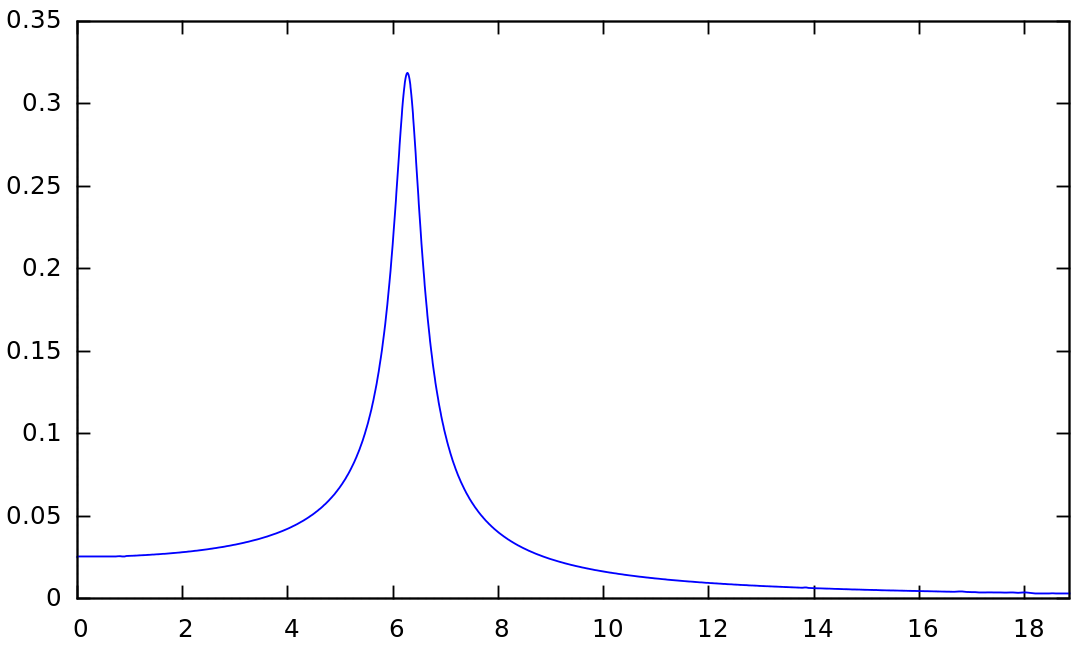
\includegraphics[width=.55\textwidth]{resonantie_curve}
	\end{image}
	\captionof{figure}{$A$ in functie van $\omega$.}
	De frequentie waarbij dit optreedt noemen we de \emph{resonantiefrequentie}. Het systeem zal dus bij \'e\'en specifieke frequentie extreem meetrillen. Op de juiste momenten wordt er dus aan de massa geduwd/getrokken zodat er maximaal energie wordt `ingepompt'. Die energie gaat dan natuurlijk weer verloren door de demping.
	
\end{document}
